\documentclass[11pt,a4paper]{article}
\usepackage{paquete}


\begin{document}


\pagestyle{fancy}
%\renewcommand{\sectionmark}[1]{\markboth{}{\thesection\ \ #1}}
\lhead{\sc }
\chead{}
\rhead{\rightmark}
\lfoot{}
\cfoot{}
\rfoot{\thepage}

%\begin{comment}
%
% Carátula:

\begin{titlepage}

\thispagestyle{empty}

\begin{center}

\includegraphics[scale=0.5]{./figuras/logo_utn}\\
\hfill \newline
\large{\textsc{Resumen Paradigma Funcional}}\\
\large{\textsc{Facultad Regional Buenos Aires}}\\
\large{\textsc{Universidad Tecnologica Nacional}}\\
\end{center}

% \newline
\begin{center}
\LARGE{\textsc{Paradigmas de Programación -- $K2032$}}\\
\hfill \newline
\huge{Trabajos Prácticos}
\end{center}

\vspace{2cm}



\begin{center}
	\begin{tabular}{lc}
		PAZ PORTILLA, José Miguel & \ \ \ 2028244 \\
		\texttt{\href{mailto:jpazportilla@frba.utn.edu.ar}{jpazportilla@frba.utn.edu.ar}}\\
	\end{tabular}
\end{center}

\vspace{1cm}
\begin{center}
\large{\today}
\end{center}

\end{titlepage}

%
% Pongo el índice en una página aparte:
%
{
  \hypersetup{linkcolor=black}
  \tableofcontents
}
% \tableofcontents
\thispagestyle{empty}
\newpage
%
% Hago que las páginas se comiencen a contar a partir de aquí:
%
\setcounter{page}{1}



\newpage
%%%%%%%%%%%%%%%%%%%%%%%%%%%%%%%%%%%%%%%%%%%%%%%%%%%%%%%%%%%%%%%%%%%%%%%

\section{Introducción a Lógico -> Video 10 Youtube}

En prolog se deben escribir predicados en un archivo con extensión .pl, luego para ejecutarlo desde terminal se debe escribir swipl nombre\_archivo.pl, para salir halt., para actualizar make., para correr test run\_test.

La cantidad de parametros que recibe un predicado se llama aridad. Un predicado puede estar constituido por un hecho o bien por una regla. Donde los hechos no tienen pre requerimiento sino que es algo definido como verdadero, las reglas separan el nombre del predicado con un :- y a su derecha los pre requerimientos que debe cumplirse.

Los parametros pueden ser individuos/átomos que empieza con minuscula o bien pueden ser una Variable que empieza con mayúscula.

\subsection{$maestro\_alumno.pl$}
\lstinputlisting[]{ClaseVideo10/maestro_alumno.pl} 

Se observa que el predicado humano esta contituido por 3 hechos de aridad 1, el predicado mortal por 1 regla y 1 hecho de aridad 1, el predicado maestro por 2 hechos de aridad 2, el predicado groso por 1 regla de aridad 1.

\begin{figure}[H]
	\centering
	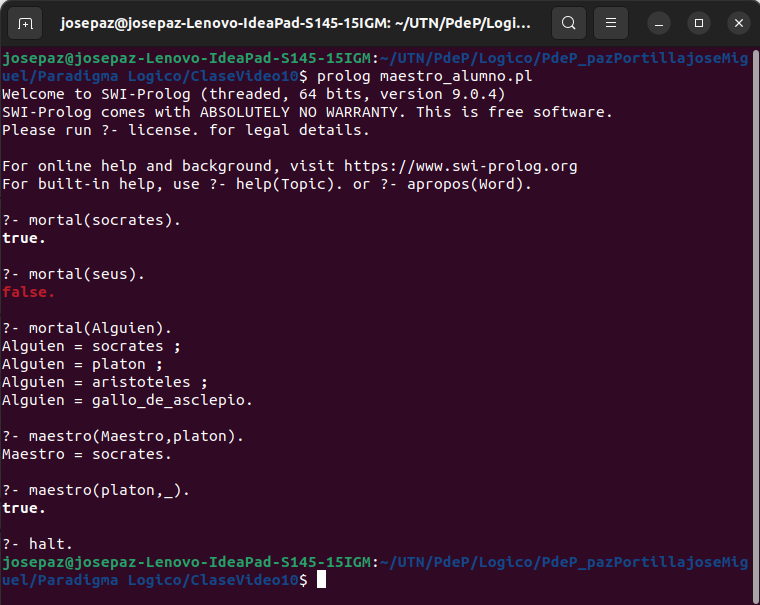
\includegraphics[scale=0.6]{figuras/maestro_alumno.png}
    \caption{Consultas a prolog con base de conocimiento maestro\_alumno.pl}
    \label{fig:maestro alumno}
\end{figure} 



%%%%%%%%%%%%%%%%%%%%%%%%%%%%%%%%%%%%%%%%%%%%%%%%%%%%%%%%%%%%%%%%%%%% 
\newpage

\appendix

%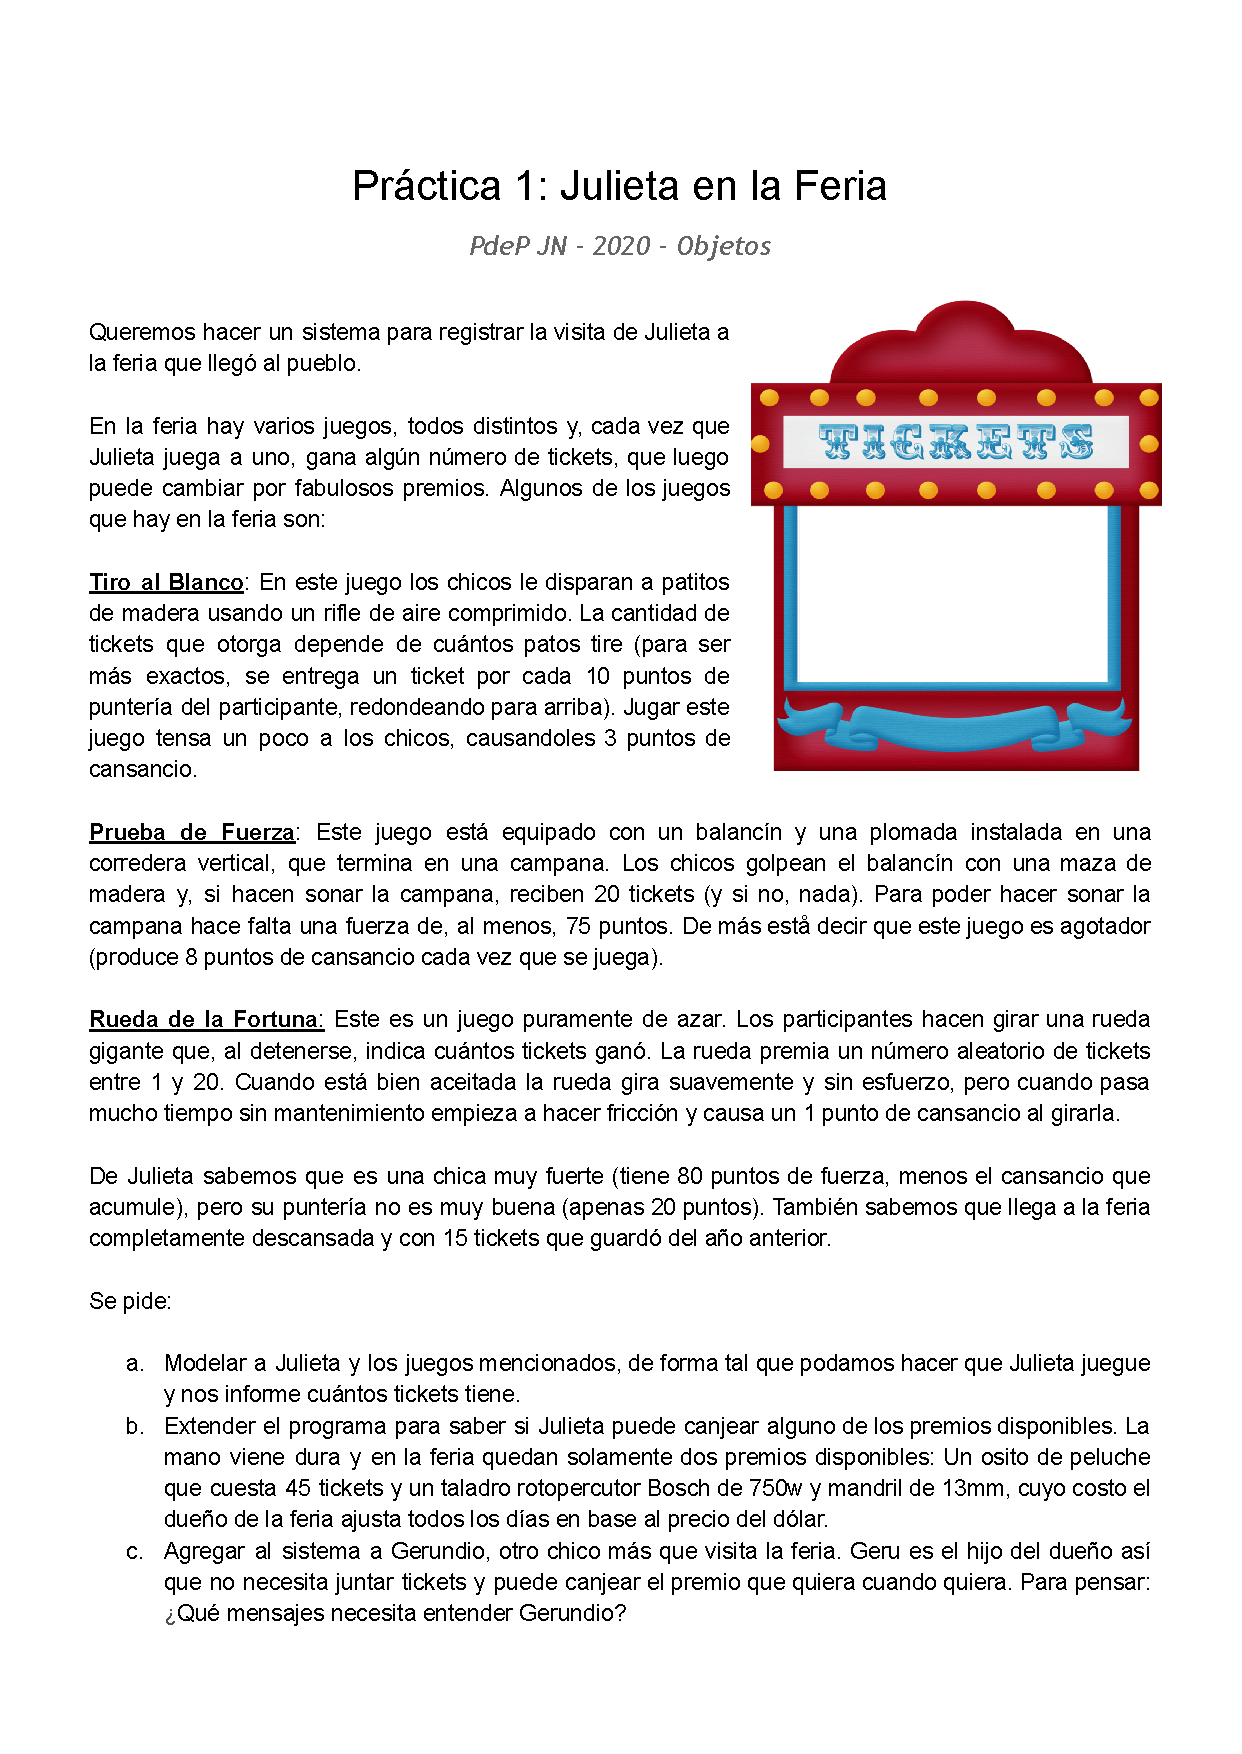
\includepdf[pages=-]{LaFeriaVideo18.pdf}
%\lstinputlisting[]{codigos/video17_e1_pepita/src/pepita.wlk}
%\lstinputlisting{codigo.asm}

\end{document}
